\documentclass{beamer}

\usepackage{hyperref}
\hypersetup{
  pdfinfo={
    CreationDate={D:20180702102722},
    ModDate={D:20180702102722},
  },
}

\AtBeginSection[]
{
  \begin{frame}
    \frametitle{Table of Contents}
    \tableofcontents[currentsection]
  \end{frame}
}

\usetheme{metropolis}
% Some configurations of metropolis theme
\metroset{block=fill}
\metroset{numbering=none}
% Set some custom colors for the beamer theme
\definecolor{DarkBlue}{HTML}{163a7a}
\definecolor{jr@medblue}{RGB}{103,169,207}
\definecolor{jr@green}{RGB}{77,175,74}
\definecolor{jr@darkred}{RGB}{153,0,0}
\setbeamercolor{frametitle}{bg=DarkBlue}
\setbeamercolor{progress bar}{fg=black}
\setbeamercolor{progress bar}{bg=black}
\setbeamercolor{background canvas}{bg=white}
% Use serif font for math
\usefonttheme[onlymath]{serif}
% Margins
\setbeamersize{text margin left=0.5cm,text margin right=0.5cm}
% Slide footer (optional)
\setbeamertemplate{footline}[text line]{%
\parbox{\linewidth}{\vspace*{-0.5cm}\small\hspace{11.15cm}%
\parbox{1cm}{\raggedleft\scriptsize\insertframenumber}}}
\setbeamertemplate{navigation symbols}{}

% lmss uses the computer modern tt font, better for URLs, etc.
\newcommand{\lmss}{\fontfamily{lmtt}\selectfont}
\newcommand{\eps}{\varepsilon}

\title[Lagrange and B\'{e}zier]
  {High-order Solution Transfer between Curved Meshes and
  Ill-conditioned B\'{e}zier Curve Intersection}
\date{August 9, 2018}
\author{Danny Hermes}
\institute{{\lmss dhermes@berkeley.edu} \\
           UC Berkeley}
\titlegraphic{
  \vspace{5cm}\hfill
  
\includegraphics[height=1.5cm]{uc_berkeley_seal.pdf}
  \hspace{1.5cm}
}

\begin{document}

\maketitle

%%%%%%%%%%%%%%%%%%%%%%%%%%%%%%%%%%%%%%%%%%%%%%%%%%%%%%%%%%%%%%%%%%%%%%%%%%%%%%%%
%%%   OUTLINE   %%%%%%%%%%%%%%%%%%%%%%%%%%%%%%%%%%%%%%%%%%%%%%%%%%%%%%%%%%%%%%%%
%%%%%%%%%%%%%%%%%%%%%%%%%%%%%%%%%%%%%%%%%%%%%%%%%%%%%%%%%%%%%%%%%%%%%%%%%%%%%%%%
\begin{frame}
\centering
{\Large\bf Outline} \\
\rule{0.82\textwidth}{1pt} \\[20pt]
\begin{minipage}{0.78\textwidth}\raggedright
\begin{enumerate}
\item Introduction and motivation
\item Solution Transfer
\item Compensated Evaluation
\item Modified Newton's for Intersection
\end{enumerate}
\end{minipage}
\end{frame}

%%%%%%%%%%%%%
%%% INTRO %%%
%%%%%%%%%%%%%

\begin{frame}
\centering
{\Large \bf Introduction and motivation}
\rule{0.82\textwidth}{1pt}
\end{frame}

\begin{frame}
\frametitle{Method of Characteristics}
\pause
Solve simple transport equation
\begin{equation*}
u_t + c u_x = 0, \quad u(x, 0) = u_0(x).
\end{equation*}
\pause
Divide physical domain
\begin{equation*}
x(t) = x_0 + ct
\end{equation*}
\pause
PDE becomes a (trivial) ODE
\begin{equation*}
\frac{d}{dt} u(x(t), t) = 0.
\end{equation*}
\end{frame}

\begin{frame}
\frametitle{Method of Characteristics}
\begin{center}
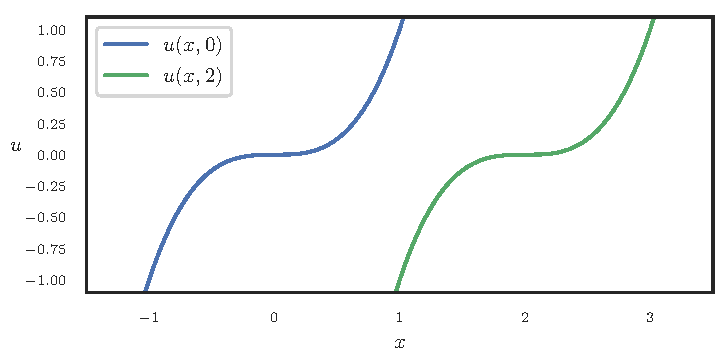
\includegraphics[width=0.95\textwidth]
                {../images/solution-transfer/simple_transport.pdf}
\end{center}
\end{frame}

\begin{frame}
\frametitle{Lagrangian Methods}
\begin{itemize}
\pause
\item Each point in the physical domain is a \textbf{particle}
\pause
\item Carry value (e.g. heat, pressure, density) along characteristic curve
\pause
\item Transform PDE to family of ODEs
\end{itemize}
\end{frame}

\begin{frame}
\frametitle{Lagrangian Methods}
\pause
Add viscosity term to transport equation
\begin{equation*}
u_t + c u_x - \eps u_{xx} = 0.
\end{equation*}
\pause
Same characteristics used, \textbf{but} solution no
longer constant
\pause
\begin{equation*}
\frac{d}{dt} u(x(t), t) = \eps u_{xx}.
\end{equation*}
\end{frame}

\begin{frame}
\frametitle{Remeshing and Adaptivity}
\begin{itemize}
\item Problems caused by flow-based mesh changes
\begin{itemize}
\pause
\item Distortion
\pause
\item Tangling
\pause
\item Travel outside relevant physical domain
\end{itemize}
\pause
\item Adaptivity
\begin{itemize}
\pause
\item Dynamically focus computational effort
\pause
\item Resolve sensitive features
\end{itemize}
\end{itemize}
\end{frame}

\begin{frame}
\frametitle{Remeshing Example}
Consider
\begin{equation*}
u_t + \left[ \begin{array}{c} y^2 \\ 1 \end{array}\right] \cdot \nabla u +
  F\left(u, \nabla u\right) = 0
\end{equation*}
\pause
with cubic characteristics
\begin{equation*}
\left[ \begin{array}{c} x(t) \\ y(t) \end{array}\right] =
  \left[ \begin{array}{c} x_0 \\ y_0 \end{array}\right] +
  \frac{1}{3} \left[ \begin{array}{c} (y_0 + t)^3 - y_0^3 \\
  3t \end{array}\right].
\end{equation*}
\end{frame}

\begin{frame}
\frametitle{Remeshing Example}
\begin{center}
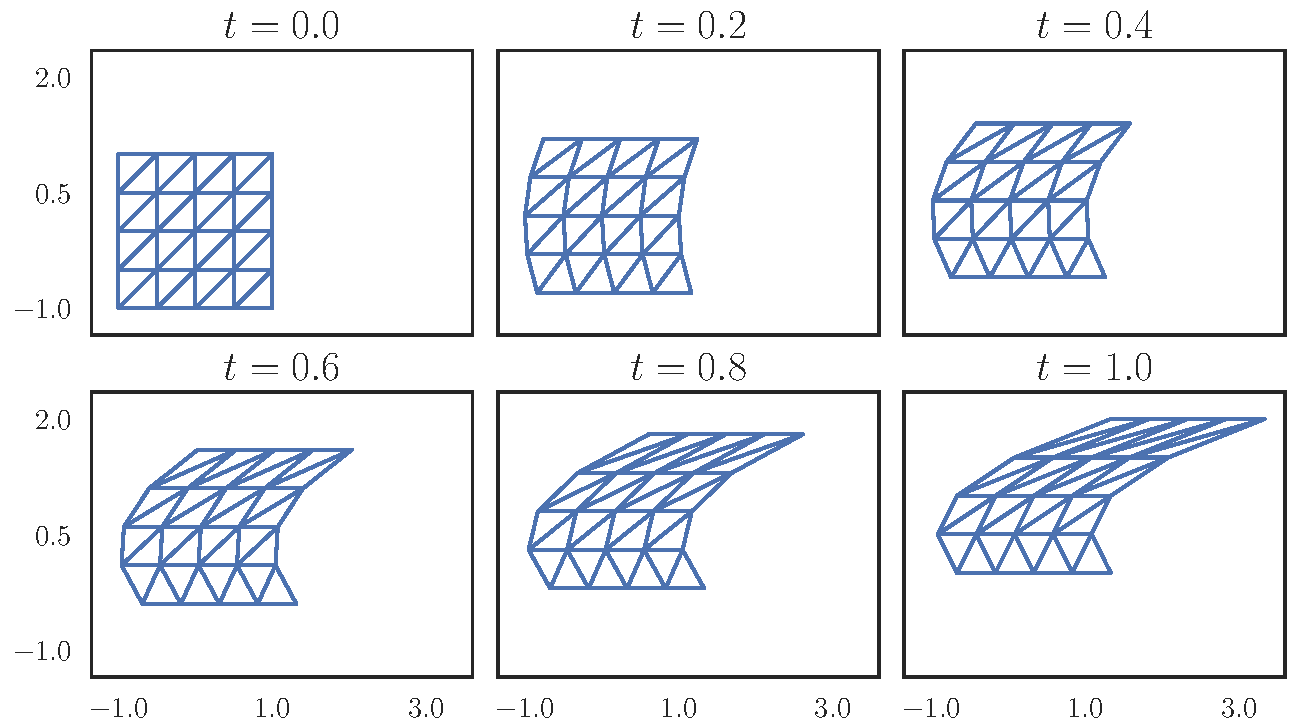
\includegraphics[width=0.95\textwidth]
                {../images/slides/mesh_distortion.pdf}
\end{center}
\end{frame}

\begin{frame}
\frametitle{Remeshing Example}
\begin{center}
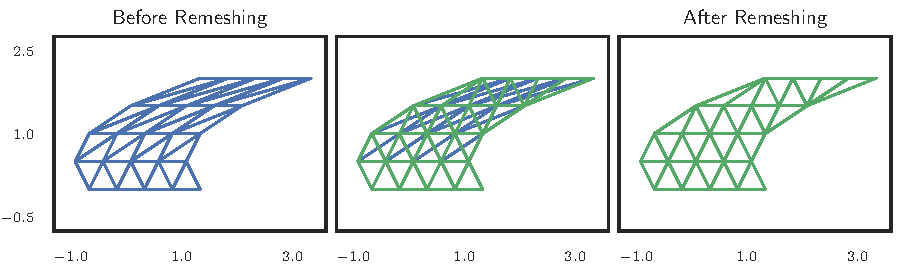
\includegraphics[width=0.95\textwidth]
                {../images/solution-transfer/distortion_remesh.pdf}
\end{center}
\end{frame}

\begin{frame}
\frametitle{High-order Meshes}
%% H/T: https://stackoverflow.com/a/4684091/1068170
\begin{center}
\includegraphics<1>[width=0.95\textwidth]
                   {../images/slides/element_distortion1.pdf}
\includegraphics<2>[width=0.95\textwidth]
                   {../images/slides/element_distortion2.pdf}
\includegraphics<3>[width=0.95\textwidth]
                   {../images/slides/element_distortion3.pdf}
\end{center}
\end{frame}

%%%%%%%%%%%%%%%%%%%%%%%%%
%%% SOLUTION TRANSFER %%%
%%%%%%%%%%%%%%%%%%%%%%%%%

\begin{frame}
\centering
{\Large \bf Solution Transfer}
\rule{0.82\textwidth}{1pt}
\end{frame}

%%%%%%%%%%%%%%%%%%%%%%%%%%%%%%
%%% COMPENSATED EVALUATION %%%
%%%%%%%%%%%%%%%%%%%%%%%%%%%%%%

\begin{frame}
\centering
{\Large \bf Compensated Evaluation}
\rule{0.82\textwidth}{1pt}
\end{frame}

%%%%%%%%%%%%%%%%%%%%%%%%%%%%%%%%%%%%%%%%%%
%%% MODIFIED NEWTON'S FOR INTERSECTION %%%
%%%%%%%%%%%%%%%%%%%%%%%%%%%%%%%%%%%%%%%%%%

\begin{frame}
\centering
{\Large \bf Modified Newton's for Intersection}
\rule{0.82\textwidth}{1pt}
\end{frame}

\begin{frame}
\frametitle{Difficulties with Curved Elements}
\begin{center}
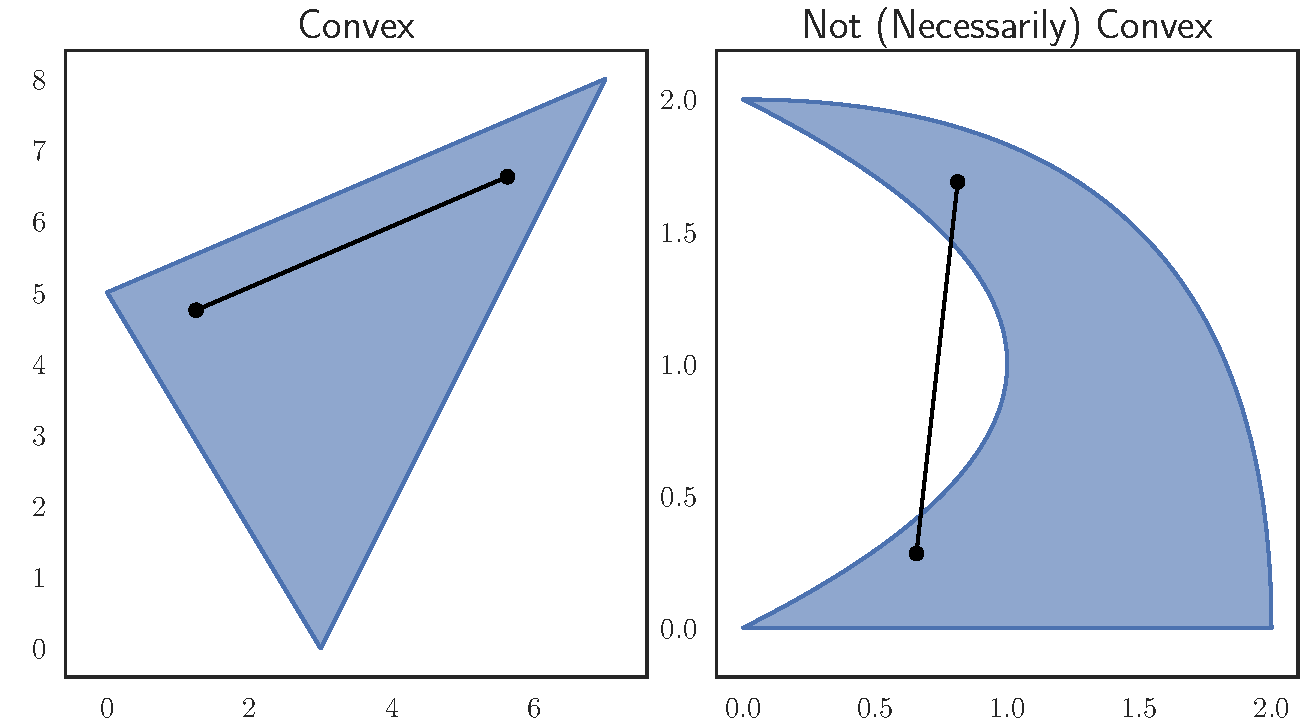
\includegraphics[width=0.95\textwidth]
                {../images/slides/not_convex.pdf}
\end{center}
\end{frame}

\begin{frame}
\frametitle{Difficulties with Curved Elements}
\begin{center}
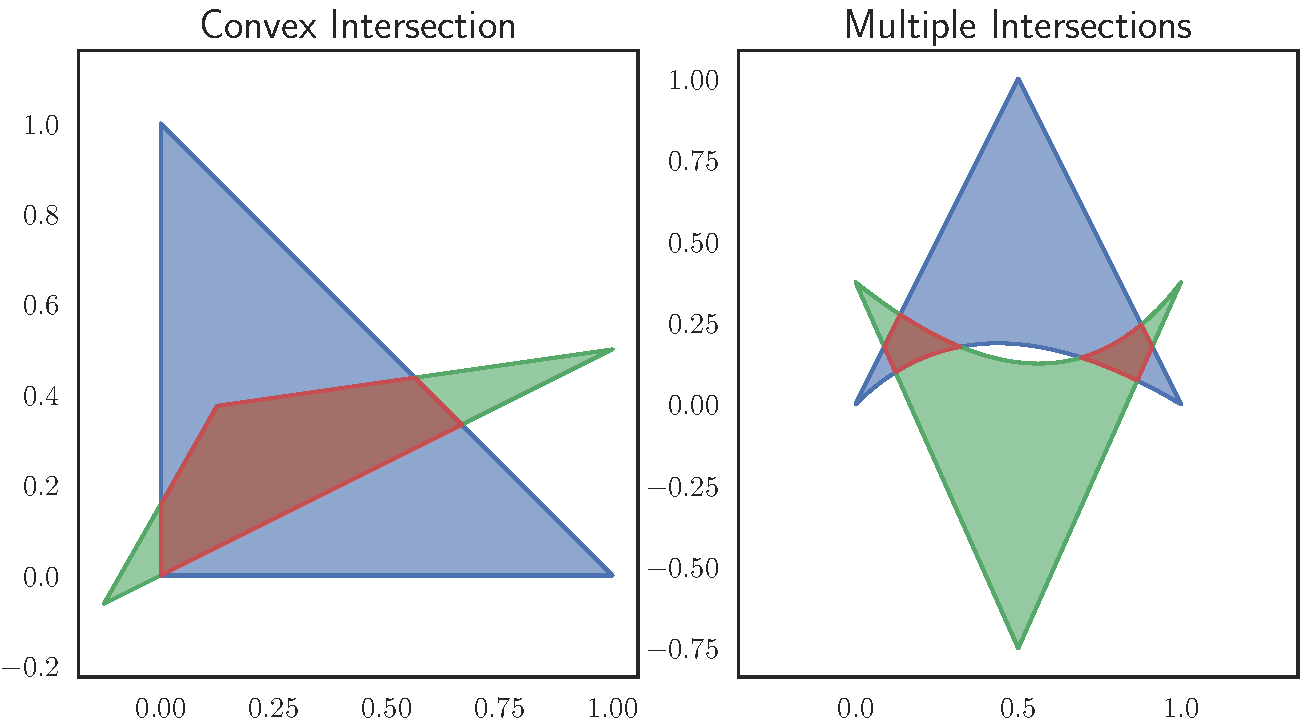
\includegraphics[width=0.95\textwidth]
                {../images/slides/split_intersection.pdf}
\end{center}
\end{frame}

\end{document}
